\documentclass{article}

% content/resources/templates/preamble.tex
\usepackage[margin=0.6in]{geometry}
\author{Milav Dabgar}
\usepackage{amsmath,amssymb,amsthm}
\usepackage{booktabs}
\usepackage{multirow}
\usepackage{xcolor}
\usepackage{tcolorbox}
\tcbuselibrary{breakable,skins}
\usepackage[colorlinks=true,linkcolor=blue]{hyperref}
\usepackage{titlesec}
\usepackage{enumitem}
\usepackage{tikz}
\usepackage{pgfplots}
\usepackage{circuitikz}
\usepackage[version=4]{mhchem}
\usepackage{longtable}
\usepackage{array}
\usepackage{float}
\usepackage{caption}
\usepackage{listings}

\lstset{
  basicstyle=\small\ttfamily,
  breaklines=true,
  breakatwhitespace=false,
  postbreak=\mbox{\textcolor{red}{$\hookrightarrow$}\space},
  float=false,
  numbers=left,
  numberstyle=\tiny\color{gray},
  numbersep=10pt,
  xleftmargin=2em,
  keywordstyle=\color{blue},
  commentstyle=\color{green!60!black},
  stringstyle=\color{purple},
  backgroundcolor=\color{gray!5},
  showstringspaces=false,
  tabsize=2,
  captionpos=b,
  keepspaces=true,
  columns=flexible
}

\pgfplotsset{compat=1.18}
\usetikzlibrary{shapes,arrows,positioning,calc,patterns,decorations.pathmorphing,decorations.markings,arrows.meta}

% Color scheme
\definecolor{headcolor}{RGB}{0,102,204}
\definecolor{keycolor}{RGB}{220,20,60}
\definecolor{solutioncolor}{RGB}{34,139,34}
\definecolor{mnemoniccolor}{RGB}{148,0,211}
\definecolor{codecolor}{RGB}{0,0,100}

% Spacing
\setlength{\parskip}{3pt}
\setlist[itemize]{nosep}
\setlist[enumerate]{nosep}

% Title formatting
\titleformat{\section}{\Large\bfseries\color{headcolor}}{\thesection}{1em}{}
\titleformat{\subsection}{\large\bfseries\color{headcolor}}{\thesubsection}{1em}{}

% Pandoc tightlist compatibility
\providecommand{\tightlist}{%
  \setlength{\itemsep}{0pt}\setlength{\parskip}{0pt}}

% Pandoc longtable compatibility
\newcounter{none}
\def\thenone{}


% content/resources/templates/english-boxes.tex

% Custom environments
\newtcolorbox{solutionbox}{
 breakable,
 enhanced,
 colback=solutioncolor!5!white,
 colframe=solutioncolor!75!black,
 fonttitle=\bfseries,
 title=Solution
}

\newtcolorbox{solutionboxnobreak}{
 colback=solutioncolor!5!white,
 colframe=solutioncolor!75!black,
 fonttitle=\bfseries,
 title=Solution
}

\newtcolorbox{keyformula}{
 breakable,
 enhanced,
 colback=keycolor!5!white,
 colframe=keycolor!75!black,
 fonttitle=\bfseries,
 title=Key Formula
}

\newtcolorbox{mnemonicboxenv}{
 breakable,
 enhanced,
 colback=mnemoniccolor!5!white,
 colframe=mnemoniccolor!75!black,
 fonttitle=\bfseries,
 title=Mnemonic
}

\newcommand{\mnemonicbox}[1]{%
  \begin{mnemonicboxenv}
    #1
  \end{mnemonicboxenv}
}


% Custom commands for GTU solutions
% This file defines semantic commands for consistent formatting

% Question command with automatic formatting
\newcommand{\question}[2]{%
  \section*{Question #1}%
  \textbf{#2}%
}

% OR question variant
\newcommand{\questionor}[2]{%
  \section*{Question #1 OR}%
  \textbf{#2}%
}

% Proper table environment with caption
\newenvironment{answertable}[1]{%
  \begin{table}[htbp]
  \centering
  \caption{#1}
}{%
  \end{table}
}

% Proper figure environment for diagrams
\newenvironment{answerdiagram}[1]{%
  \begin{figure}[htbp]
  \centering
  \caption{#1}
}{%
  \end{figure}
}

% Semantic markup for key terms
\newcommand{\keyword}[1]{\textbf{#1}}
\newcommand{\code}[1]{\texttt{#1}}
\newcommand{\classname}[1]{\texttt{#1}}
\newcommand{\methodname}[1]{\texttt{#1}}

% Proper quotation marks
\newcommand{\mnemonic}[1]{``#1''}


\title{VLSI Technology (4361102) - Summer 2025 Solution}
\date{May 12 , 2025}

\begin{document}
\maketitle

% Question 1
\questionmarks{1(a)}{3}{State importance of scaling}
\begin{solutionbox}
Scaling is crucial for advancing semiconductor technology and improving device performance.

\begin{answertable}{Scaling Benefits}
\begin{tabulary}{\textwidth}{|L|L|}
\hline
\textbf{Scaling Benefits} & \textbf{Description} \\
\hline
\textbf{Device Size} & Reduces transistor dimensions for higher density \\
\hline
\textbf{Speed} & Faster switching due to shorter channel length \\
\hline
\textbf{Power} & Lower power consumption per operation \\
\hline
\textbf{Cost} & More chips per wafer, reducing cost per function \\
\hline
\end{tabulary}
\end{answertable}

\begin{itemize}
    \item \keyword{Technology advancement}: Enables Moore's Law continuation
    \item \keyword{Performance boost}: Higher frequency operation possible
    \item \keyword{Market competitiveness}: Smaller, faster, cheaper products
\end{itemize}
\end{solutionbox}

\begin{mnemonicbox}
\mnemonic{Small Devices Speed Progress Cheaply}
\end{mnemonicbox}

\questionmarks{1(b)}{4}{Compare Planar MOSFET and FINFET}
\begin{solutionbox}
FinFET technology addresses limitations of planar MOSFET at smaller nodes.

\begin{answertable}{Planar MOSFET vs FinFET}
\begin{tabulary}{\textwidth}{|L|L|L|}
\hline
\textbf{Parameter} & \textbf{Planar MOSFET} & \textbf{FinFET} \\
\hline
\textbf{Structure} & 2D flat channel & 3D fin-shaped channel \\
\hline
\textbf{Gate Control} & Single gate & Tri-gate/multi-gate \\
\hline
\textbf{Short Channel Effects} & High at small nodes & Significantly reduced \\
\hline
\textbf{Leakage Current} & Higher subthreshold leakage & Much lower leakage \\
\hline
\end{tabulary}
\end{answertable}

\begin{itemize}
    \item \keyword{Scalability}: FinFET enables sub-22nm technology nodes
    \item \keyword{Power efficiency}: FinFET offers better power-performance ratio
    \item \keyword{Manufacturing}: FinFET requires more complex fabrication
\end{itemize}
\end{solutionbox}

\begin{mnemonicbox}
\mnemonic{Fins Control Current Better Than Flat}
\end{mnemonicbox}

\questionmarks{1(c)}{7}{Draw and Explain VDS-ID AND VGS-ID characteristics of N channel MOSFET}
\begin{solutionbox}
N-channel MOSFET characteristics show device behavior in different operating regions.

\textbf{Diagram:}

\begin{answerdiagram}{MOSFET Characteristics}
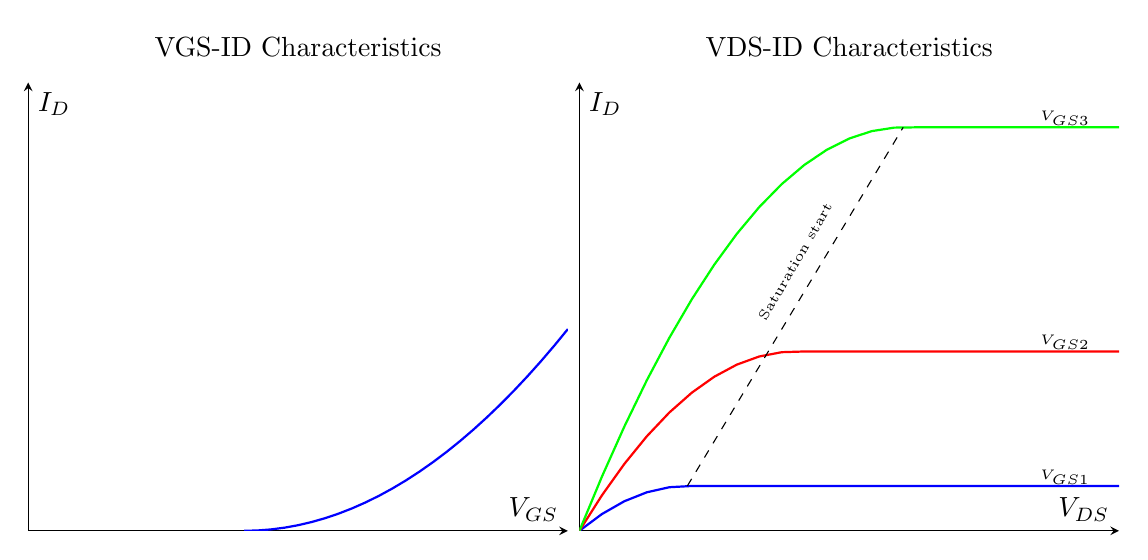
\begin{tikzpicture}
\begin{scope}
    \begin{axis}[
        title={VGS-ID Characteristics},
        xlabel={$V_{GS}$},
        ylabel={$I_D$},
        xmin=0, xmax=5,
        ymin=0, ymax=10,
        axis lines=middle,
        ticks=none
    ]
    \addplot[domain=2:5, blue, thick] {0.5*(x-2)^2};
    \node at (axis cs:2,0) [below] {$V_T$};
    \end{axis}
\end{scope}

\begin{scope}[xshift=7cm]
    \begin{axis}[
        title={VDS-ID Characteristics},
        xlabel={$V_{DS}$},
        ylabel={$I_D$},
        xmin=0, xmax=5,
        ymin=0, ymax=10,
        axis lines=middle,
        ticks=none
    ]
    \addplot[domain=0:5, blue, thick] {x < 1 ? 2*x - x^2 : 1};
    \addplot[domain=0:5, red, thick] {x < 2 ? 4*x - x^2 : 4};
    \addplot[domain=0:5, green, thick] {x < 3 ? 6*x - x^2 : 9};
    
    \node at (axis cs:4.5, 1.2) {\tiny $V_{GS1}$};
    \node at (axis cs:4.5, 4.2) {\tiny $V_{GS2}$};
    \node at (axis cs:4.5, 9.2) {\tiny $V_{GS3}$};
    
    \draw[dashed] (axis cs:1,1) -- (axis cs:3,9);
    \node at (axis cs:2, 6) [rotate=60] {\tiny Saturation start};
    \end{axis}
\end{scope}
\end{tikzpicture}
\end{answerdiagram}

\begin{answertable}{MOSFET Operating Regions}
\begin{tabulary}{\textwidth}{|L|L|L|}
\hline
\textbf{Region} & \textbf{Condition} & \textbf{Current Equation} \\
\hline
\textbf{Cutoff} & $V_{GS} < V_T$ & $I_D = 0$ \\
\hline
\textbf{Linear} & $V_{DS} < (V_{GS}-V_T)$ & $I_D \propto V_{DS}$ \\
\hline
\textbf{Saturation} & $V_{DS} \ge (V_{GS}-V_T)$ & $I_D \propto (V_{GS}-V_T)^2$ \\
\hline
\end{tabulary}
\end{answertable}

\begin{itemize}
    \item \keyword{Cutoff}: No current flows, acts as open switch.
    \item \keyword{Linear/Triode}: Current increases linearly with $V_{DS}$, acts as resistor.
    \item \keyword{Saturation}: Current is constant, independent of $V_{DS}$, acts as current source.
\end{itemize}
\end{solutionbox}

\begin{mnemonicbox}
\mnemonic{Threshold Gates Linear Saturation}
\end{mnemonicbox}

\subsubsection*{OR}

\subsection*{(c) Explain different condition of MOS under external bias [7 marks]}
\textbf{Answer:}
External bias creates different charge distributions affecting MOS capacitor behavior.

\textbf{Diagram:}

\begin{figure}[H]
\centering
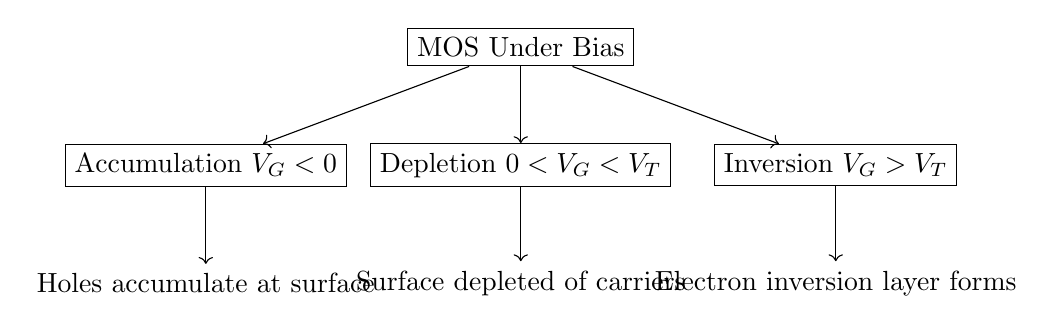
\begin{tikzpicture}[node distance=1.5cm]
    \node (mos) [draw, rectangle] {MOS Under Bias};
    
    \node (acc) [draw, rectangle, below of=mos, xshift=-4cm] {Accumulation $V_G < 0$};
    \node (dep) [draw, rectangle, below of=mos] {Depletion $0 < V_G < V_T$};
    \node (inv) [draw, rectangle, below of=mos, xshift=4cm] {Inversion $V_G > V_T$};
    
    \node (acc_desc) [below of=acc] {Holes accumulate at surface};
    \node (dep_desc) [below of=dep] {Surface depleted of carriers};
    \node (inv_desc) [below of=inv] {Electron inversion layer forms};
    
    \draw[->] (mos) -- (acc);
    \draw[->] (mos) -- (dep);
    \draw[->] (mos) -- (inv);
    
    \draw[->] (acc) -- (acc_desc);
    \draw[->] (dep) -- (dep_desc);
    \draw[->] (inv) -- (inv_desc);
\end{tikzpicture}
\caption{MOS Bias Modes}
\end{figure}

\begin{table}[H]
\centering
\begin{tabulary}{\textwidth}{|L|L|L|}
\hline
\textbf{Bias Condition} & \textbf{Surface State} & \textbf{Capacitance} \\
\hline
\textbf{Accumulation} & Majority carriers at surface & High ($C_{ox}$) \\
\hline
\textbf{Depletion} & No mobile carriers & Medium \\
\hline
\textbf{Inversion} & Minority carriers form channel & High ($C_{ox}$) \\
\hline
\end{tabulary}
\end{table}

\begin{itemize}
    \item \textbf{Flat band voltage}: No charge separation exists
    \item \textbf{Energy band bending}: Determines carrier distribution
    \item \textbf{Surface potential}: Controls inversion layer formation
\end{itemize}

\begin{mnemonicbox}[Mnemonic]
"Accumulate, Deplete, then Invert"
\end{mnemonicbox}


% Question 2
\questionmarks{2(a)}{3}{Draw voltage transfer characteristic of ideal inverter}
\begin{solutionbox}
Ideal inverter provides sharp transition between logic levels with infinite gain.

\textbf{Diagram:}

\begin{answerdiagram}{Ideal Inverter VTC}
\begin{tikzpicture}
    \begin{axis}[
        title={Ideal Inverter VTC},
        xlabel={$V_{IN}$},
        ylabel={$V_{OUT}$},
        xmin=0, xmax=5,
        ymin=0, ymax=5,
        axis lines=middle,
        ticks=none,
        width=8cm, height=8cm
    ]
    % Ideal VTC
    \draw[blue, thick] (axis cs:0,5) -- (axis cs:2.5,5) -- (axis cs:2.5,0) -- (axis cs:5,0);
    
    \node at (axis cs:0,5) [left] {$V_{OH}$};
    \node at (axis cs:5,0) [below] {$V_{OL}$};
    \node at (axis cs:2.5,0) [below] {$V_{TH}$};
    
    \draw[dashed] (axis cs:1,0) -- (axis cs:1,5);
    \node at (axis cs:1,0) [below] {$V_{IL}$};
    
    \draw[dashed] (axis cs:4,0) -- (axis cs:4,5);
    \node at (axis cs:4,0) [below] {$V_{IH}$};

    \end{axis}
\end{tikzpicture}
\end{answerdiagram}

\begin{itemize}
    \item \keyword{Sharp transition}: Infinite slope at switching point
    \item \keyword{Noise margins}: $NMH = V_{OH} - V_{IH}$, $NML = V_{IL} - V_{OL}$
    \item \keyword{Perfect logic levels}: $V_{OH} = V_{DD}$, $V_{OL} = 0V$
\end{itemize}
\end{solutionbox}

\begin{mnemonicbox}
\mnemonic{Sharp Switch, Perfect Levels}
\end{mnemonicbox}

\questionmarks{2(b)}{4}{Explain noise immunity and noise margin}
\begin{solutionbox}
Noise immunity measures circuit's ability to reject unwanted signal variations.

\begin{answertable}{Noise Margin Parameters}
\begin{tabulary}{\textwidth}{|L|L|L|}
\hline
\textbf{Parameter} & \textbf{Definition} & \textbf{Formula} \\
\hline
\textbf{NMH} & High-level noise margin & $V_{OH} - V_{IH}$ \\
\hline
\textbf{NML} & Low-level noise margin & $V_{IL} - V_{OL}$ \\
\hline
\textbf{Noise Immunity} & Ability to reject noise & $Min(NMH, NML)$ \\
\hline
\end{tabulary}
\end{answertable}

\begin{itemize}
    \item \keyword{Logic threshold levels}: $V_{IH}$ (input high), $V_{IL}$ (input low)
    \item \keyword{Output levels}: $V_{OH}$ (output high), $V_{OL}$ (output low)
    \item \keyword{Better immunity}: Larger noise margins provide better protection
    \item \keyword{Design goal}: Maximize noise margins for robust operation
\end{itemize}
\end{solutionbox}

\begin{mnemonicbox}
\mnemonic{Margins Protect Against Noise}
\end{mnemonicbox}

\questionmarks{2(c)}{7}{Describe inverter circuit with saturated and linear depletion load nMOS inverter}
\begin{solutionbox}
Depletion load nMOS inverters use depletion transistor as active load resistor.

\textbf{Diagram:}

\begin{answerdiagram}{Depletion Load Inverter}
\begin{circuitikz}[american]
    % Depletion Load NMOS Inverter
    \draw (0,0) node[ground] {} to[nmos, n=driver, l=MN (Driver)] (0,2);
    
    % Load NMOS (Depletion mode simulated with nmos)
    \draw (0,2) -- (0,2.5) to[nmos, n=load, l=MD (Depletion)] (0,4.5) node[vcc] {VDD};
    
    % Depletion thick channel
    \draw[thick] ($(load.source)!0.5!(load.drain)$) ++(-0.2,0) -- ++(0,0.6); % Rough sketch of depletion line if needed
    
    % Connections
    \draw (load.gate) -- ++(-0.5,0) -- ++(0,0) coordinate (gd);
    \draw (gd) |- (load.source); % VGS=0 for depletion load
    
    \draw (driver.gate) to[short,-o] (-1,0.5) node[left] {$V_{IN}$};
    \draw (0,2.25) to[short,*-o] (2,2.25) node[right] {$V_{OUT}$};
    
\end{circuitikz}
\end{answerdiagram}

\begin{answertable}{Load Types}
\begin{tabulary}{\textwidth}{|L|L|L|}
\hline
\textbf{Load Type} & \textbf{Gate Connection} & \textbf{Operation} \\
\hline
\textbf{Saturated Load} & $V_G = V_D$ & Always in saturation \\
\hline
\textbf{Linear Load} & $V_G = V_{DD}$ & Can operate in linear region \\
\hline
\end{tabulary}
\end{answertable}

\begin{itemize}
    \item \keyword{Depletion device}: Conducts with $V_{GS} = 0$, acts as current source
    \item \keyword{Load line analysis}: Determines operating point intersection
    \item \keyword{Power consumption}: Always conducting, higher static power
    \item \keyword{Switching speed}: Faster pull-down than pull-up
\end{itemize}
\end{solutionbox}

\begin{mnemonicbox}
\mnemonic{Depletion Loads Drive Outputs}
\end{mnemonicbox}

\begin{center}
\textbf{\large OR}
\end{center}

\questionmarks{2(a)}{3}{Draw and explain enhancement load inverter}
\begin{solutionbox}
Enhancement load inverter uses enhancement MOSFET as load with special biasing.

\textbf{Diagram:}

\begin{answerdiagram}{Enhancement Load Inverter}
\begin{circuitikz}
    \draw (0,0) node[ground] {} to[nmos, n=driver] (0,2);
    \draw (0,2) -- (0,2.5) to[nmos, n=load] (0,4.5) node[vcc] {VDD};
    
    % Diode connected load (Enhancement)
    \draw (load.gate) -- (load.drain);
    \draw (load.gate) ++(0,0) node[circ] {};
    
    % Input/Output
    \draw (driver.gate) to[short,-o] (-1,1) node[left] {$V_{IN}$};
    \draw (0,2.25) to[short,*-o] (1.5,2.25) node[right] {$V_{OUT}$};
    
    % Labels
    \node[right] at (driver) {Driver};
    \node[right] at (load) {Enhancement Load};
\end{circuitikz}
\end{answerdiagram}

\begin{itemize}
    \item \keyword{Bootstrap connection}: Gate connected to drain for load
    \item \keyword{Limited output high}: $V_{OUT(max)} = V_{DD} - V_T$
    \item \keyword{Threshold loss}: Enhancement load causes voltage drop
\end{itemize}
\end{solutionbox}

\begin{mnemonicbox}
\mnemonic{Enhancement Loses Threshold}
\end{mnemonicbox}

\questionmarks{2(b)}{4}{List the advantages of CMOS inverter}
\begin{solutionbox}
CMOS technology offers superior performance compared to NMOS inverters.

\begin{answertable}{CMOS Advantages}
\begin{tabulary}{\textwidth}{|L|L|}
\hline
\textbf{Advantage} & \textbf{Benefit} \\
\hline
\textbf{Zero static power} & No current path in steady state \\
\hline
\textbf{Rail-to-rail output} & Full $V_{DD}$ and 0V output levels \\
\hline
\textbf{High noise immunity} & Large noise margins \\
\hline
\textbf{Symmetric switching} & Equal rise and fall times \\
\hline
\end{tabulary}
\end{answertable}

\begin{itemize}
    \item \keyword{Power efficiency}: Only dynamic power during switching
    \item \keyword{Scalability}: Works well at all technology nodes
    \item \keyword{Fan-out capability}: Can drive multiple inputs
    \item \keyword{Temperature stability}: Performance less sensitive to temperature
\end{itemize}
\end{solutionbox}

\begin{mnemonicbox}
\mnemonic{CMOS Saves Power Perfectly}
\end{mnemonicbox}

\questionmarks{2(c)}{7}{Draw and Explain operating mode of region for CMOS Inverter}
\begin{solutionbox}
CMOS inverter operation involves five distinct regions based on input voltage.

\textbf{Diagram:}

\begin{answerdiagram}{CMOS Operation Regions}
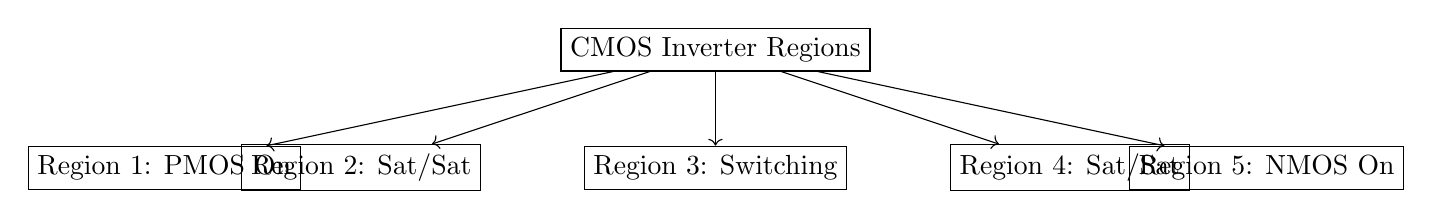
\begin{tikzpicture}[node distance=1.5cm]
    \node (cmos) [draw, rectangle] {CMOS Inverter Regions};
    
    \node (reg3) [draw, rectangle, below of=cmos] {Region 3: Switching};
    \node (reg2) [draw, rectangle, left of=reg3, xshift=-3cm] {Region 2: Sat/Sat};
    \node (reg1) [draw, rectangle, left of=reg2, xshift=-1cm] {Region 1: PMOS On};
    \node (reg4) [draw, rectangle, right of=reg3, xshift=3cm] {Region 4: Sat/Sat};
    \node (reg5) [draw, rectangle, right of=reg4, xshift=1cm] {Region 5: NMOS On};
    
    \draw[->] (cmos) -- (reg3);
    \draw[->] (cmos) -- (reg2);
    \draw[->] (cmos) -- (reg1);
    \draw[->] (cmos) -- (reg4);
    \draw[->] (cmos) -- (reg5);
    
\end{tikzpicture}
\end{answerdiagram}

\begin{answertable}{CMOS Operating Regions}
\begin{tabulary}{\textwidth}{|L|L|L|L|}
\hline
\textbf{Region} & \textbf{NMOS State} & \textbf{PMOS State} & \textbf{Output} \\
\hline
\textbf{1} & OFF & Linear & $V_{OH} \approx V_{DD}$ \\
\hline
\textbf{2} & Saturation & Saturation & Transition \\
\hline
\textbf{3} & Saturation & Saturation & $V_{DD}/2$ \\
\hline
\textbf{4} & Saturation & Saturation & Transition \\
\hline
\textbf{5} & Linear & OFF & $V_{OL} \approx 0V$ \\
\hline
\end{tabulary}
\end{answertable}

\begin{itemize}
    \item \keyword{Switching threshold}: VTC crosses $V_{DD}/2$ at region 3
    \item \keyword{Current flow}: Only during transition regions 2,3,4
    \item \keyword{Noise margins}: Regions 1 and 5 provide immunity
    \item \keyword{Gain}: Maximum in region 3 (switching point)
\end{itemize}
\end{solutionbox}

% Question 3
\questionmarks{3(a)}{3}{Draw two input NOR gate using CMOS}
\begin{solutionbox}
CMOS NOR gate implements De Morgan's law using complementary networks.

\textbf{Diagram:}

\begin{answerdiagram}{CMOS NOR2 Gate}
\begin{circuitikz}
    % PUN: Series PMOS
    \draw (0,4) node[vcc] {VDD} to[Tpmos, name=p1, l=MP1 (A)] (0,3);
    \draw (0,3) to[Tpmos, name=p2, l=MP2 (B)] (0,2);
    
    % PDN: Parallel NMOS
    \draw (0,2) -- (0,1.5);
    \draw (-1.5,1.5) -- (1.5,1.5);
    \draw (-1.5,1.5) to[Tnmos, name=n1, l=MN1 (A)] (-1.5,0.5);
    \draw (1.5,1.5) to[Tnmos, name=n2, l=MN2 (B)] (1.5,0.5);
    \draw (-1.5,0.5) -- (1.5,0.5);
    \draw (0,0.5) -- (0,0) node[ground] {};
    
    % Output
    \draw (0,2) to[short, *-o] (2.5,2) node[right] {$Y = \overline{A+B}$};
    
    % Input Connections
    \draw (p1.gate) -- ++(-1,0) node[left] {A};
    \draw (n1.gate) -- ++(-0.5,0) node[left] {A};
    \draw (p2.gate) -- ++(-1,0) node[left] {B};
    \draw (n2.gate) -- ++(0.5,0) node[right] {B};
\end{circuitikz}
\end{answerdiagram}

\begin{itemize}
    \item \keyword{Pull-up network}: Series PMOS transistors (A AND B both low for high output)
    \item \keyword{Pull-down network}: Parallel NMOS transistors (A OR B high for low output)
    \item \keyword{Logic function}: $Y = (A+B)' = A' \cdot B'$
\end{itemize}
\end{solutionbox}

\begin{mnemonicbox}
\mnemonic{Series PMOS, Parallel NMOS}
\end{mnemonicbox}

\questionmarks{3(b)}{4}{Implement Boolean function Z= [(A+B)C+DE]' using CMOS}
\begin{solutionbox}
Complex CMOS logic uses AOI (AND-OR-Invert) structure for efficient implementation.

\textbf{Diagram:}

\begin{answerdiagram}{CMOS Implementation of $Z = [(A+B)C+DE]'$}
\begin{circuitikz}
    % PDN
    \draw (0,0) node[ground] {} -- (0,0.5);
    % Branch 1: D series E
    \draw (0,0.5) -- (2,0.5) to[Tnmos, l=E] (2,1.5) to[Tnmos, l=D] (2,2.5) -- (0,2.5);
    
    % Branch 2: (A || B) series C
    \draw (0,0.5) -- (-2,0.5) to[Tnmos, l=C] (-2,1.5);
    % Parallel A, B
    \draw (-2,1.5) -- (-3,1.5) to[Tnmos, l=A] (-3,2.5) -- (-2,2.5);
    \draw (-2,1.5) -- (-1,1.5) to[Tnmos, l=B] (-1,2.5) -- (-2,2.5);
    \draw (-2,2.5) -- (0,2.5);
    
    % Output node
    \draw (0,2.5) to[short, *-o] (3,2.5) node[right] {Z};
    
    % PUN: Dual of PDN
    \draw (0,2.5) -- (0,3);
    
    % Block 2: D || E
    \draw (0,3) -- (-1,3) to[Tpmos, l=D] (-1,4) -- (0,4);
    \draw (0,3) -- (1,3) to[Tpmos, l=E] (1,4) -- (0,4);
    
    % Block 1: (A series B) || C
    \draw (0,4) -- (0,4.5);
    % Path C
    \draw (0,4.5) -- (1.5,4.5) to[Tpmos, l=C] (1.5,6.5) -- (0,6.5);
    % Path A series B
    \draw (0,4.5) -- (-1.5,4.5) to[Tpmos, l=B] (-1.5,5.5) to[Tpmos, l=A] (-1.5,6.5) -- (0,6.5);
    
    \draw (0,6.5) node[vcc] {VDD};
    
\end{circuitikz}
\end{answerdiagram}

\begin{itemize}
    \item \keyword{AOI structure}: Efficient single-stage implementation
    \item \keyword{Dual networks}: Complementary pull-up and pull-down
    \item \keyword{Logic optimization}: Fewer transistors than separate gates
\end{itemize}
\end{solutionbox}

\begin{mnemonicbox}
\mnemonic{AOI Inverts Complex Logic Efficiently}
\end{mnemonicbox}

\questionmarks{3(c)}{7}{Draw and explain CMOS NAND2 gate with the parasitic device capacitances}
\begin{solutionbox}
Parasitic capacitances in CMOS gates affect switching speed and power consumption.

\textbf{Diagram:}

\begin{answerdiagram}{CMOS NAND2 with Parasitics}
\begin{circuitikz}
    % CMOS NAND2
    % Parallel PMOS
    \draw (0,5) node[vcc] {VDD} -- (0,4.5);
    \draw (-1.5,4.5) -- (1.5,4.5);
    \draw (-1.5,4.5) to[Tpmos, l=MP1] (-1.5,3);
    \draw (1.5,4.5) to[Tpmos, l=MP2] (1.5,3);
    \draw (-1.5,3) -- (1.5,3);
    \draw (0,3) -- (0,2.5);
    
    % Series NMOS
    \draw (0,2.5) to[Tnmos, l=MN2] (0,1.5);
    \draw (0,1.5) to[Tnmos, l=MN1] (0,0.5) node[ground] {};
    
    % Output
    \draw (0,2.75) to[short, *-o] (3,2.75) node[right] {$Y$};
    
    % Parasitic Capacitors
    \draw (-1.5,4) to[C, l=$C_{gd1}$, color=red] (-0.5,4);
    \draw (1.5,4) to[C, l=$C_{gd2}$, color=red] (0.5,4);
    
    % Load Cap
    \draw (2.5,2.75) to[C, l=$C_{load}$, color=red] (2.5,0.5) node[ground] {};
    
    % Cgs, Cdb etc can be indicated generally or specific nodes
    \node[right, red] at (0.5, 1) {$C_{gd}, C_{db}$};
    
\end{circuitikz}
\end{answerdiagram}

\begin{answertable}{Parasitic Capacitances}
\begin{tabulary}{\textwidth}{|L|L|L|}
\hline
\textbf{Capacitance} & \textbf{Location} & \textbf{Effect} \\
\hline
\textbf{Cgs} & Gate-Source & Input capacitance \\
\hline
\textbf{Cgd} & Gate-Drain & Miller effect \\
\hline
\textbf{Cdb} & Drain-Bulk & Output loading \\
\hline
\textbf{Csb} & Source-Bulk & Source loading \\
\hline
\end{tabulary}
\end{answertable}

\begin{itemize}
    \item \keyword{Switching delay}: Parasitic capacitances slow transitions
    \item \keyword{Power consumption}: Charging/discharging parasitic caps
    \item \keyword{Miller effect}: Cgd creates feedback, slows switching
    \item \keyword{Layout optimization}: Minimize parasitic capacitances
\end{itemize}
\end{solutionbox}

\begin{mnemonicbox}
\mnemonic{Parasitics Slow Gates Down}
\end{mnemonicbox}

\begin{center}
\textbf{\large OR}
\end{center}

\questionmarks{3(a)}{3}{Draw and explain NOR based Clocked SR latch using CMOS}
\begin{solutionbox}
Clocked SR latch uses NOR gates with clock enable for synchronous operation.

\textbf{Diagram:}

\begin{answerdiagram}{Clocked SR Latch}
\begin{circuitikz}
    \node[nor port] (nor1) at (0,2) {};
    \node[nor port] (nor2) at (0,-2) {};
    
    % Input NORs for Clock gating
    \node[and port] (and1) at (-3, 2.3) {}; % Actually logic is usually AND-NOR or just extra inputs to NOR?
    % The question says "NOR based". Usually means SR latch (cross coupled NORs) with AND gates for clock, OR simply NORs with clock?
    % Standard implementation: S connects to AND with CLK, output to NOR latch.
    % Let's use logic gates for clarity.
    
    \node[and port] (gate1) at (-3, 2) {};
    \node[and port] (gate2) at (-3, -2) {};
    
    \node[nor port] (latch1) at (0, 1.5) {};
    \node[nor port] (latch2) at (0, -1.5) {};
    
    % Connections
    \draw (gate1.out) -- (latch1.in 1);
    \draw (gate2.out) -- (latch2.in 2);
    
    % Cross coupling
    \draw (latch1.out) -- ++(0.5,0) coordinate (q) -- ++(0,-1) -- ($(latch2.in 1) + (-0.5, 1.5)$) -- (latch2.in 1);
    \draw (latch2.out) -- ++(0.5,0) coordinate (qb) -- ++(0,1) -- ($(latch1.in 2) + (-0.5, -1.5)$) -- (latch1.in 2);
    
    % Inputs
    \draw (gate1.in 1) -- ++(-0.5,0) node[left] {S};
    \draw (gate2.in 2) -- ++(-0.5,0) node[left] {R};
    
    % Clock
    \draw (gate1.in 2) -- ++(-0.5,0) coordinate (clk1);
    \draw (gate2.in 1) -- ++(-0.5,0) coordinate (clk2);
    \draw (clk1) -- (clk2); 
    \draw ($(clk1)!0.5!(clk2)$) -- ++(-1,0) node[left] {CLK};
    
    % Outputs
    \draw (latch1.out) -- ++(1,0) node[right] {Q};
    \draw (latch2.out) -- ++(1,0) node[right] {Q'};
    
\end{circuitikz}
\end{answerdiagram}

\begin{itemize}
    \item \keyword{Clock control}: S and R effective only when CLK = 1
    \item \keyword{Transparent mode}: Output follows input when clock active
    \item \keyword{Hold mode}: Output maintains state when clock inactive
    \item \keyword{Basic building block}: Foundation for flip-flops
\end{itemize}
\end{solutionbox}

\begin{mnemonicbox}
\mnemonic{Clock Controls Transparent Latching}
\end{mnemonicbox}

\questionmarks{3(b)}{4}{Implement Boolean function Z=[AB+C(D+E)]' using CMOS}
\begin{solutionbox}
This function implements inverted sum-of-products using AOI logic structure.

\textbf{Logic Analysis:}
$Z = [AB + C(D+E)]' = [AB + CD + CE]'$

\textbf{Diagram:}

\begin{answerdiagram}{CMOS Implementation of $Z=[AB+C(D+E)]'$}
\begin{circuitikz}
    % PDN: AB + C(D+E) as per equation
    % (A series B) || (C series (D || E))
    \draw (0,0) node[ground] {} -- (0,0.5);
    
    % Branch 1: A series B
    \draw (0,0.5) -- (-2,0.5) to[Tnmos, l=B] (-2,1.5) to[Tnmos, l=A] (-2,2.5) -- (0,2.5);
    
    % Branch 2: C series (D || E)
    \draw (0,0.5) -- (2,0.5);
    % D || E
    \draw (2,0.5) -- (1,0.5) to[Tnmos, l=D] (1,1.5) -- (2,1.5);
    \draw (2,0.5) -- (3,0.5) to[Tnmos, l=E] (3,1.5) -- (2,1.5);
    % Series C
    \draw (2,1.5) to[Tnmos, l=C] (2,2.5) -- (0,2.5);
    
    % Output
    \draw (0,2.5) to[short, *-o] (3,2.5) node[right] {Z};
    
    % PUN: Dual of PDN
    \draw (0,2.5) -- (0,3);
    
    % Block 1: A || B
    \draw (0,3) -- (-1.5,3) to[Tpmos, l=A] (-1.5,4) -- (0,4);
    \draw (0,3) -- (1.5,3) to[Tpmos, l=B] (1.5,4) -- (0,4);
    
    % Block 2: C || (D series E)
    \draw (0,4) -- (0,4.5);
    % Path C
    \draw (0,4.5) -- (-1.5,4.5) to[Tpmos, l=C] (-1.5,6.5) -- (0,6.5);
    % Path D series E
    \draw (0,4.5) -- (1.5,4.5) to[Tpmos, l=E] (1.5,5.5) to[Tpmos, l=D] (1.5,6.5) -- (0,6.5);
    
    \draw (0,6.5) node[vcc] {VDD};
    
\end{circuitikz}
\end{answerdiagram}

\begin{answertable}{Boolean Terms}
\begin{tabulary}{\textwidth}{|L|L|L|}
\hline
\textbf{Term} & \textbf{Inputs} & \textbf{Function} \\
\hline
\textbf{Term 1} & A, B & AB \\
\hline
\textbf{Term 2} & C, D & CD \\
\hline
\textbf{Term 3} & C, E & CE \\
\hline
\textbf{Output} & All terms & (AB + CD + CE)' \\
\hline
\end{tabulary}
\end{answertable}

\begin{itemize}
    \item \keyword{AOI implementation}: Single stage, efficient design
    \item \keyword{Transistor count}: Fewer than separate gate implementation
    \item \keyword{Performance}: Fast switching, low power
\end{itemize}
\end{solutionbox}

\begin{mnemonicbox}
\mnemonic{Three AND Terms Feed One NOR}
\end{mnemonicbox}

\questionmarks{3(c)}{7}{Differentiate AOI and OAI Logic with example}
\begin{solutionbox}
AOI and OAI are complementary logic families for efficient CMOS implementation.

\begin{answertable}{AOI vs OAI}
\begin{tabulary}{\textwidth}{|L|L|L|}
\hline
\textbf{Parameter} & \textbf{AOI (AND-OR-Invert)} & \textbf{OAI (OR-AND-Invert)} \\
\hline
\textbf{Structure} & AND gates $\rightarrow$ OR $\rightarrow$ Invert & OR gates $\rightarrow$ AND $\rightarrow$ Invert \\
\hline
\textbf{Function} & $(AB + CD + ...)'$ & $((A+B)(C+D)...)'$ \\
\hline
\textbf{PMOS Network} & Series-parallel & Parallel-series \\
\hline
\textbf{NMOS Network} & Parallel-series & Series-parallel \\
\hline
\end{tabulary}
\end{answertable}

\textbf{AOI Example: $Y = (AB + CD)'$}
\begin{itemize}
    \item PMOS: Series A-B in parallel with Series C-D
    \item NMOS: Parallel A,B in series with Parallel C,D
\end{itemize}

\textbf{OAI Example: $Y = ((A+B)(C+D))'$}
\begin{itemize}
    \item PMOS: Parallel A,B in series with Parallel C,D
    \item NMOS: Series A-B in parallel with Series C-D
\end{itemize}

\begin{itemize}
    \item \keyword{Design choice}: Select based on Boolean function form
    \item \keyword{Optimization}: Minimizes transistor count and delay
    \item \keyword{Duality}: AOI and OAI are De Morgan duals
\end{itemize}
\end{solutionbox}

\begin{mnemonicbox}
\mnemonic{AOI ANDs then ORs, OAI ORs then ANDs}
\end{mnemonicbox}

% Question 4
\questionmarks{4(a)}{3}{Define: 1) Regularity 2) Modularity 3) Locality}
\begin{solutionbox}
Design hierarchy principles essential for managing VLSI complexity and ensuring successful implementation.

\begin{answertable}{Design Principles}
\begin{tabulary}{\textwidth}{|L|L|L|}
\hline
\textbf{Principle} & \textbf{Definition} & \textbf{Benefit} \\
\hline
\textbf{Regularity} & Repeated use of similar structures & Easier layout, testing \\
\hline
\textbf{Modularity} & Breaking design into smaller blocks & Independent design, reuse \\
\hline
\textbf{Locality} & Interconnections mostly local & Reduced routing complexity \\
\hline
\end{tabulary}
\end{answertable}

\begin{itemize}
    \item \keyword{Design efficiency}: Principles reduce design time and effort
    \item \keyword{Verification}: Modular approach simplifies testing
    \item \keyword{Scalability}: Enables larger, more complex designs
\end{itemize}
\end{solutionbox}

\begin{mnemonicbox}
\mnemonic{Regular Modules Stay Local}
\end{mnemonicbox}

\questionmarks{4(b)}{4}{Implement SR latch (NAND gate) using CMOS inverter}
\begin{solutionbox}
SR latch using NAND gates provides set-reset functionality with active-low inputs.

\textbf{Diagram:}

\begin{answerdiagram}{NAND SR Latch}
\begin{circuitikz}
    \node[nand port] (nand1) at (0,2) {};
    \node[nand port] (nand2) at (0,-2) {};
    
    % Cross coupling
    \draw (nand1.out) -- ++(0.5,0) coordinate (q) -- ++(0,-1.5) -- ($(nand2.in 1) + (-0.5, 1)$) -- (nand2.in 1);
    \draw (nand2.out) -- ++(0.5,0) coordinate (qb) -- ++(0,1.5) -- ($(nand1.in 2) + (-0.5, -1)$) -- (nand1.in 2);
    
    % Inputs
    \draw (nand1.in 1) -- ++(-1,0) node[left] {S'};
    \draw (nand2.in 2) -- ++(-1,0) node[left] {R'};
    
    % Outputs
    \draw (nand1.out) -- ++(1,0) node[right] {Q};
    \draw (nand2.out) -- ++(1,0) node[right] {Q'};
\end{circuitikz}
\end{answerdiagram}

\begin{answertable}{SR Latch Truth Table}
\begin{tabulary}{\textwidth}{|C|C|C|C|L|}
\hline
\textbf{S'} & \textbf{R'} & \textbf{Q} & \textbf{Q'} & \textbf{State} \\
\hline
0 & 1 & 1 & 0 & Set \\
\hline
1 & 0 & 0 & 1 & Reset \\
\hline
1 & 1 & Q & Q' & Hold \\
\hline
0 & 0 & 1 & 1 & Invalid \\
\hline
\end{tabulary}
\end{answertable}

\begin{itemize}
    \item \keyword{Cross-coupled structure}: Provides memory function
    \item \keyword{Active-low inputs}: S' = 0 sets, R' = 0 resets
    \item \keyword{Forbidden state}: Both inputs low simultaneously
\end{itemize}
\end{solutionbox}

\begin{mnemonicbox}
\mnemonic{Cross-Coupled NANDS Remember State}
\end{mnemonicbox}

\questionmarks{4(c)}{7}{Explain VLSI design flow}
\begin{solutionbox}
VLSI design flow follows systematic steps from specification to fabrication.

\textbf{Diagram:}

\begin{answerdiagram}{VLSI Design Flow}
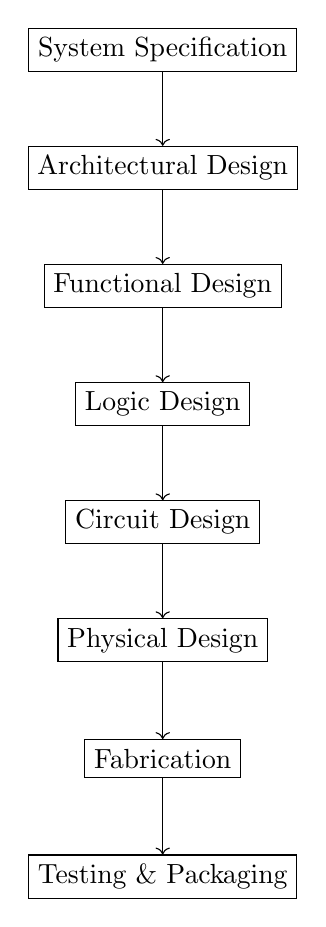
\begin{tikzpicture}[node distance=1.5cm, auto]
    \node (spec) [draw, rectangle, align=center] {System Specification};
    \node (arch) [draw, rectangle, below of=spec] {Architectural Design};
    \node (func) [draw, rectangle, below of=arch] {Functional Design};
    \node (logic) [draw, rectangle, below of=func] {Logic Design};
    \node (circuit) [draw, rectangle, below of=logic] {Circuit Design};
    \node (phys) [draw, rectangle, below of=circuit] {Physical Design};
    \node (fab) [draw, rectangle, below of=phys] {Fabrication};
    \node (test) [draw, rectangle, below of=fab] {Testing \& Packaging};
    
    \draw[->] (spec) -- (arch);
    \draw[->] (arch) -- (func);
    \draw[->] (func) -- (logic);
    \draw[->] (logic) -- (circuit);
    \draw[->] (circuit) -- (phys);
    \draw[->] (phys) -- (fab);
    \draw[->] (fab) -- (test);
\end{tikzpicture}
\end{answerdiagram}

\begin{answertable}{Design Steps}
\begin{tabulary}{\textwidth}{|L|L|L|}
\hline
\textbf{Level} & \textbf{Activities} & \textbf{Output} \\
\hline
\textbf{System} & Requirements analysis & Specifications \\
\hline
\textbf{Architecture} & Block-level design & System architecture \\
\hline
\textbf{Logic} & Boolean optimization & Gate netlist \\
\hline
\textbf{Circuit} & Transistor sizing & Circuit netlist \\
\hline
\textbf{Physical} & Layout, routing & GDSII file \\
\hline
\end{tabulary}
\end{answertable}

\begin{itemize}
    \item \keyword{Design verification}: Each level requires validation
    \item \keyword{Iteration}: Feedback loops for optimization
    \item \keyword{CAD tools}: Automation essential for complex designs
    \item \keyword{Time-to-market}: Efficient flow reduces design cycle
\end{itemize}
\end{solutionbox}

\begin{mnemonicbox}
\mnemonic{System Architects Love Circuit Physical Fabrication}
\end{mnemonicbox}

\begin{center}
\textbf{\large OR}
\end{center}

\questionmarks{4(a)}{3}{Draw and explain Y-chart}
\begin{solutionbox}
Y-chart represents three design domains and their abstraction levels in VLSI design.

\textbf{Diagram:}

\begin{answerdiagram}{Gajski-Kuhn Y-Chart}
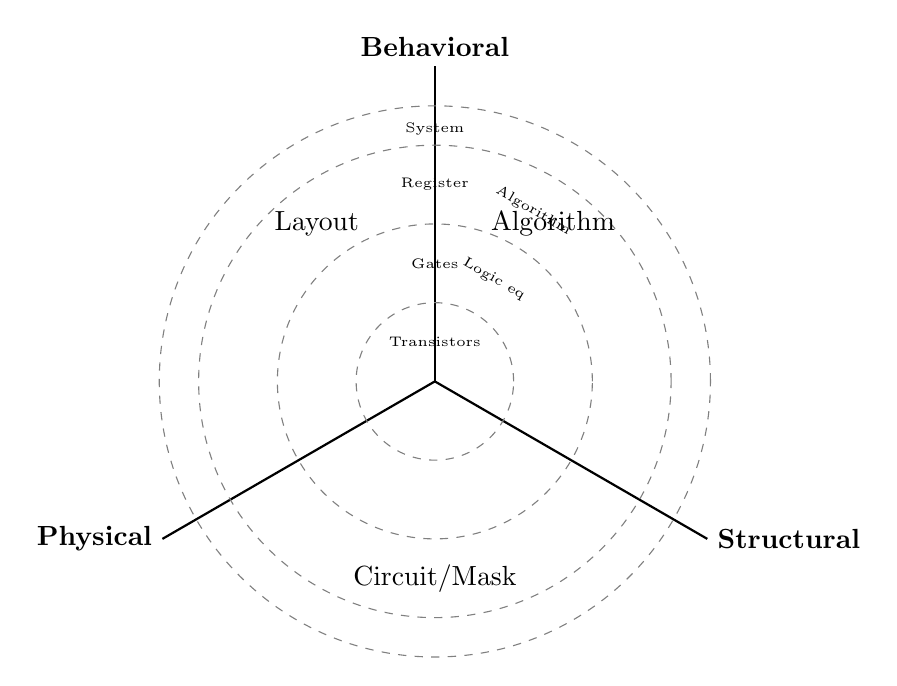
\begin{tikzpicture}
    % Y Chart Grid
    \draw[thick] (0,0) -- (0,4) node[above] {\textbf{Behavioral}};
    \draw[thick] (0,0) -- (3.46,-2) node[right] {\textbf{Structural}};
    \draw[thick] (0,0) -- (-3.46,-2) node[left] {\textbf{Physical}};
    
    % Concentric Circles (Abstraction Levels)
    \foreach \r in {1, 2, 3, 3.5}
        \draw[gray, thin, dashed] (0,0) circle (\r);
        
    % Labels (Approximate positions)
    \node at (0, 0.5) {\tiny Transistors};
    \node at (0, 1.5) {\tiny Gates};
    \node at (0, 2.5) {\tiny Register};
    \node at (0, 3.2) {\tiny System};
    
    \node at (60:1.5) [rotate=-30] {\tiny Logic eq};
    \node at (60:2.5) [rotate=-30] {\tiny Algorithm};
    
    % Add simplified labels for 3 marks
    \node[align=center] at (1.5, 2) {Algorithm};
    \node[align=center] at (-1.5, 2) {Layout};
    \node[align=center] at (0, -2.5) {Circuit/Mask};
    
\end{tikzpicture}
\end{answerdiagram}

\begin{itemize}
    \item \keyword{Three domains}: Behavioral (function), Structural (components), Physical (geometry)
    \item \keyword{Abstraction levels}: System $\rightarrow$ Algorithm $\rightarrow$ Gate $\rightarrow$ Circuit $\rightarrow$ Layout
    \item \keyword{Design methodology}: Move between domains at same abstraction level
\end{itemize}
\end{solutionbox}

\begin{mnemonicbox}
\mnemonic{Behavior, Structure, Physics at All Levels}
\end{mnemonicbox}

\questionmarks{4(b)}{4}{Implement clocked JK latch (NOR gate) using CMOS inverter}
\begin{solutionbox}
JK latch eliminates forbidden state of SR latch with toggle capability.

\textbf{Diagram:}

\begin{answerdiagram}{Clocked JK Latch}
\begin{circuitikz}
    \node[and port, number inputs=3] (and1) at (-3, 2) {};
    \node[and port, number inputs=3] (and2) at (-3, -2) {};
    
    \node[nor port] (nor1) at (0, 1) {};
    \node[nor port] (nor2) at (0, -1) {};
    
    % Inputs to AND
    \draw (and1.in 1) -- ++(-0.5,0) node[left] {J};
    \draw (and2.in 2) -- ++(-0.5,0) node[left] {K};
    \draw (and1.in 2) -- ++(-0.5,0) coordinate (clk1);
    \draw (and2.in 1) -- ++(-0.5,0) coordinate (clk2);
    \draw (clk1) -- (clk2);
    \draw ($(clk1)!0.5!(clk2)$) -- ++(-0.5,0) node[left] {CLK};
    
    % Connections AND -> NOR
    \draw (and1.out) -- (nor1.in 1);
    \draw (and2.out) -- (nor2.in 2);
    
    % Latch Feedback
    \draw (nor1.out) -- ++(0.5,0) coordinate (q) -- ++(0,-0.5) -- ($(nor2.in 1) + (-0.5, 0.5)$) -- (nor2.in 1);
    \draw (nor2.out) -- ++(0.5,0) coordinate (qb) -- ++(0,0.5) -- ($(nor1.in 2) + (-0.5, -0.5)$) -- (nor1.in 2);
    
    % JK Feedback
    \draw (qb) -- ++(0.5,0) -- ++(0,3.5) -- ++(-6,0) |- (and1.in 1);
    \draw (q) -- ++(0.5,0) -- ++(0,-3.5) -- ++(-6,0) |- (and2.in 3);
    
    % Outputs
    \draw (q) -- ++(1,0) node[right] {Q};
    \draw (qb) -- ++(1,0) node[right] {Q'};
\end{circuitikz}
\end{answerdiagram}

\begin{answertable}{JK Latch Truth Table}
\begin{tabulary}{\textwidth}{|C|C|C|L|}
\hline
\textbf{J} & \textbf{K} & \textbf{Q(next)} & \textbf{Operation} \\
\hline
0 & 0 & Q & Hold \\
\hline
0 & 1 & 0 & Reset \\
\hline
1 & 0 & 1 & Set \\
\hline
1 & 1 & Q' & Toggle \\
\hline
\end{tabulary}
\end{answertable}

\begin{itemize}
    \item \keyword{Toggle mode}: J=K=1 flips output state
    \item \keyword{Clock enable}: Active only when CLK=1
    \item \keyword{Feedback}: Uses current output to enable inputs
\end{itemize}
\end{solutionbox}

\begin{mnemonicbox}
\mnemonic{JK Toggles, No Forbidden State}
\end{mnemonicbox}

\questionmarks{4(c)}{ Explain the terms Lithography, Etching, Deposition, Oxidation, Ion implantation, Diffusion}{7}
\begin{solutionbox}
Semiconductor fabrication processes essential for creating integrated circuits.

\begin{answertable}{Fabrication Processes}
\begin{tabulary}{\textwidth}{|L|L|L|}
\hline
\textbf{Process} & \textbf{Purpose} & \textbf{Method} \\
\hline
\textbf{Lithography} & Pattern transfer & UV exposure through masks \\
\hline
\textbf{Etching} & Material removal & Wet/dry chemical processes \\
\hline
\textbf{Deposition} & Layer addition & CVD, PVD, sputtering \\
\hline
\textbf{Oxidation} & Insulator growth & Thermal/plasma oxidation \\
\hline
\textbf{Ion Implantation} & Doping introduction & High-energy ion bombardment \\
\hline
\textbf{Diffusion} & Dopant distribution & High-temperature spreading \\
\hline
\end{tabulary}
\end{answertable}

\begin{itemize}
    \item \keyword{Pattern definition}: Lithography creates device features
    \item \keyword{Selective removal}: Etching removes unwanted material
    \item \keyword{Layer building}: Deposition adds required materials
    \item \keyword{Doping control}: Implantation and diffusion create junctions
    \item \keyword{Quality control}: Each step affects final device performance
\end{itemize}
\end{solutionbox}

\begin{mnemonicbox}
\mnemonic{Light Etches Deposited Oxides, Ions Diffuse}
\end{mnemonicbox}

% Question 5
\questionmarks{5(a)}{3}{Implement 2 input XNOR gate using Verilog}
\begin{solutionbox}
XNOR gate produces high output when inputs are equal.

\begin{lstlisting}[language=Verilog, caption={Verilog Code for XNOR Gate}]
module xnor_gate(
    input a, b,
    output y
);
    assign y = ~(a ^ b);
endmodule
\end{lstlisting}

\begin{itemize}
    \item \keyword{Logic function}: $Y = (A \oplus B)' = A'B' + AB$
    \item \keyword{High Output}: When both inputs are 0 or both are 1
    \item \keyword{Applications}: Equality comparison, parity checking
\end{itemize}
\end{solutionbox}

\begin{mnemonicbox}
\mnemonic{XNOR Equals Equal Inputs}
\end{mnemonicbox}

\questionmarks{5(b)}{4}{Implement Encoder (8:3) using CASE statement in Verilog}
\begin{solutionbox}
Priority encoder converts 8-bit input to 3-bit binary output using case statement for behavioral modeling.

\begin{lstlisting}[language=Verilog, caption={8:3 Priority Encoder using CASE}]
module encoder_8to3(
    input [7:0] in,
    output reg [2:0] out
);
    always @(*) begin
        case(in)
            8'b00000001: out = 3'b000;
            8'b00000010: out = 3'b001;
            8'b00000100: out = 3'b010;
            8'b00001000: out = 3'b011;
            8'b00010000: out = 3'b100;
            8'b00100000: out = 3'b101;
            8'b01000000: out = 3'b110;
            8'b10000000: out = 3'b111;
            default: out = 3'b000;
        endcase
    end
endmodule
\end{lstlisting}

\begin{itemize}
    \item \keyword{Behavioral Modeling}: Case statement describes function conceptually
    \item \keyword{Combinational Logic}: \code{always @(*)} block used
    \item \keyword{Default case}: Handles undefined states (e.g., all zeros)
\end{itemize}
\end{solutionbox}

\begin{mnemonicbox}
\mnemonic{One Hot Input, Binary Output}
\end{mnemonicbox}

\questionmarks{5(c)}{7}{Explain CASE statement in Verilog with suitable examples}
\begin{solutionbox}
CASE statement provides multi-way branching based on expression value, typically used in combinational logic (decoders, muxes) and state machines.

\textbf{Syntax:}
\begin{lstlisting}[language=Verilog]
case (expression)
    value1: statement1;
    value2: statement2;
    default: default_statement;
endcase
\end{lstlisting}

\textbf{Example 1: 4:1 Multiplexer}
\begin{lstlisting}[language=Verilog]
module mux_4to1(
    input [1:0] sel,
    input [3:0] in,
    output reg out
);
    always @(*) begin
        case(sel)
            2'b00: out = in[0];
            2'b01: out = in[1];
            2'b10: out = in[2];
            2'b11: out = in[3];
        endcase
    end
endmodule
\end{lstlisting}

\textbf{Benefits:}
\begin{itemize}
    \item \keyword{Readability}: Clearer than multiple \code{if-else} statements
    \item \keyword{Synthesis}: Efficiently maps to multiplexers or ROMs
    \item \keyword{Parallel Evaluation}: Hardware checks all conditions simultaneously
\end{itemize}

\begin{answertable}{CASE Statement Variants}
\begin{tabulary}{\textwidth}{|L|L|L|}
\hline
\textbf{Variant} & \textbf{Syntax} & \textbf{Usage} \\
\hline
\textbf{case} & \code{case(expr)} & Exact bit matching (0, 1, x, z) \\
\hline
\textbf{casex} & \code{casex(expr)} & Treats 'x' and 'z' as don't care \\
\hline
\textbf{casez} & \code{casez(expr)} & Treats 'z' as don't care \\
\hline
\end{tabulary}
\end{answertable}
\end{solutionbox}

\begin{mnemonicbox}
\mnemonic{CASE Chooses Actions Systematically Everywhere}
\end{mnemonicbox}

\end{document}




